% Make listings font size smaller for input and output files
\lstset{basicstyle=\ttfamily\footnotesize, columns=fullflexible, keepspaces=true}
\section{Benchmarks}
The accuracy and robustness of the code is tested by solving some sample 
problems, the exact solutions of which were computed apriori via the classical
beam theory. The results are presented in this section using the following scheme: 
\begin{itemize}
    \item Demonstration of the problem
    \item Input file that addresses the problem
    \item Output file generated by the program after analysis
    \item Diagrams obtaned by postprocessing 
    \item Comparison of the results of numerical and analytical solutions
\end{itemize}
Each problem considered in the first part comprise a single or continous beam 
subjected to  a certain external loading and support condition. The second part 
deals with a one-bay one-storey frame under different loads and restraints, 
and the third and final part is devoted to problems involving a prestressed beam,
with each problem having different tendon layouts and/or support conditions.
\par
The error in each numerical solution is presented by using the true
percent relative error according to the following definition:
\begin{equation*}
    \epsilon_{r,t} = \frac{|exact \: value - numerical \: value|}
                          {|exact \: value|} \times 100
\end{equation*}
%
% PART I: BEAM BENCHMARKS
%
\subsection{Single Beam Under Various Loading and Support Conditions}
%
% PROBLEM 1
%
\subsubsection{Problem 1: Simple Beam - Uniformly Distributed Load}
\begin{figure}[h]
    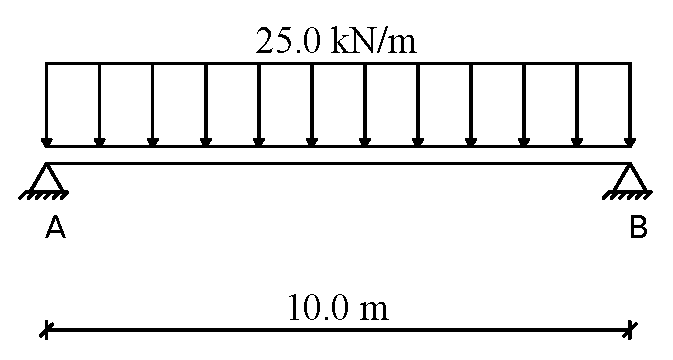
\includegraphics[width=\textwidth, keepaspectratio]{%
                            bm_figures/turtle_figures/bm01_turtle.pdf}
    \centering
    \caption{Problem 1: Loading, geometry and supports}
    \label{fig:bm01_turtle}
\end{figure}
\lstinputlisting{input_files/bm01_input.dat}
\lstinputlisting{output_files/bm01_output.dat}
% Deformed
\begin{figure}[!htb]
    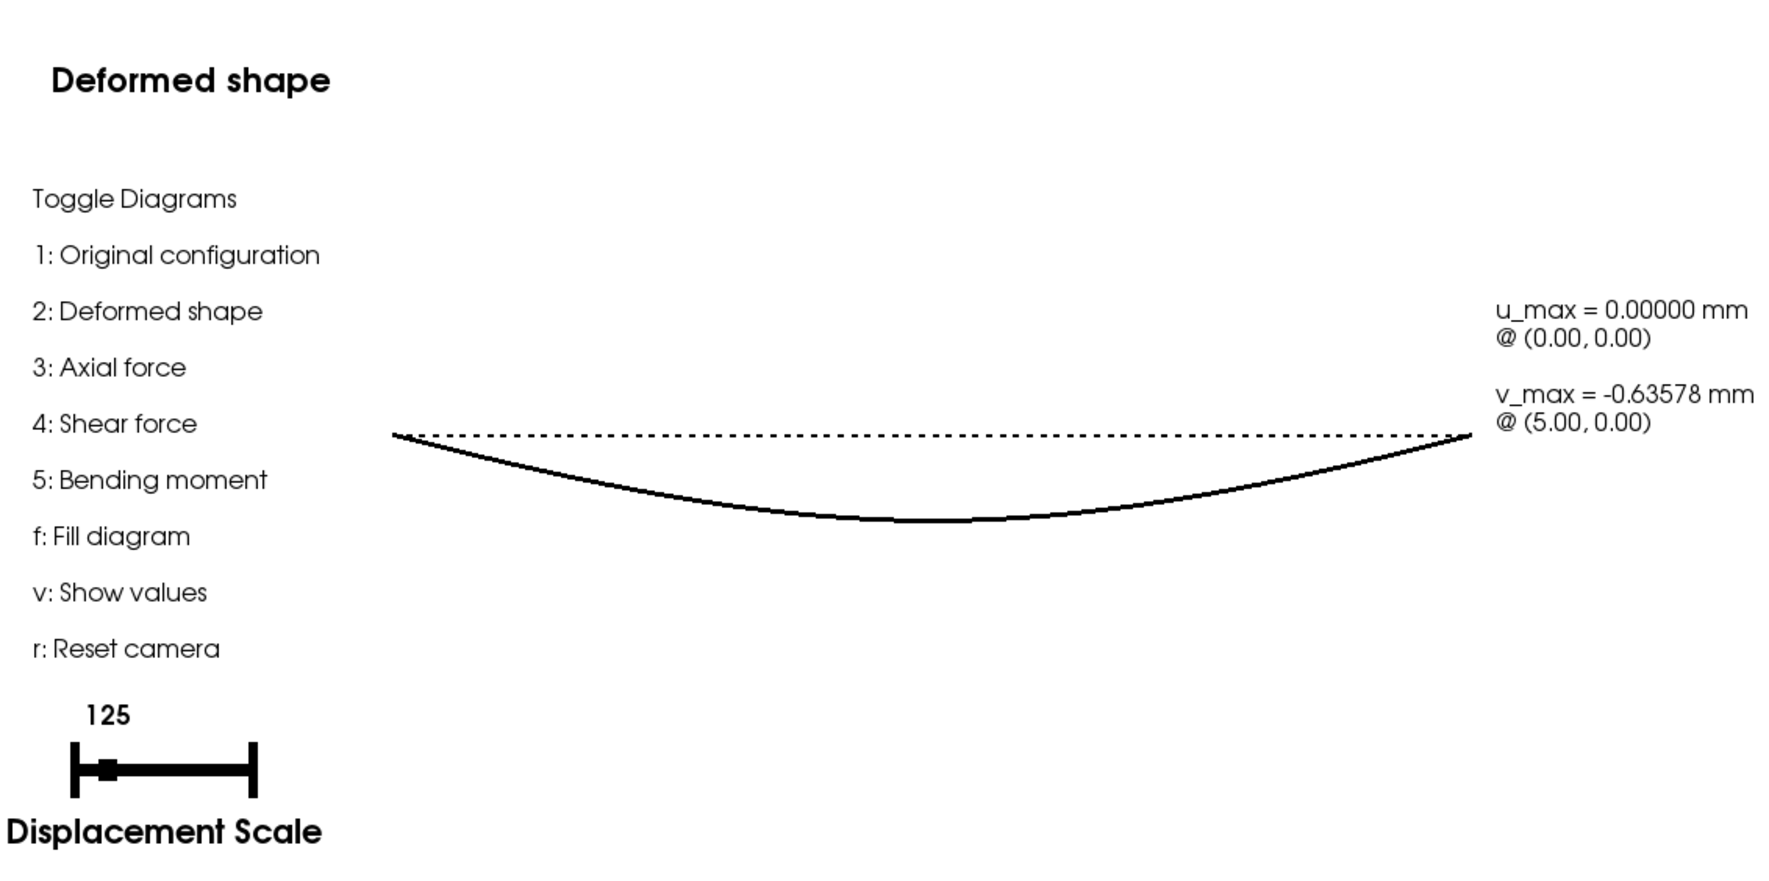
\includegraphics[width=\textwidth, keepaspectratio]{%
                     bm_figures/vtk_figures/bm01_deformed.pdf}
    \centering
    \caption{Problem 1, Deformed Shape}
    \label{fig:bm01_deformed}
\end{figure}
% Shear
\begin{figure}[!htb]
    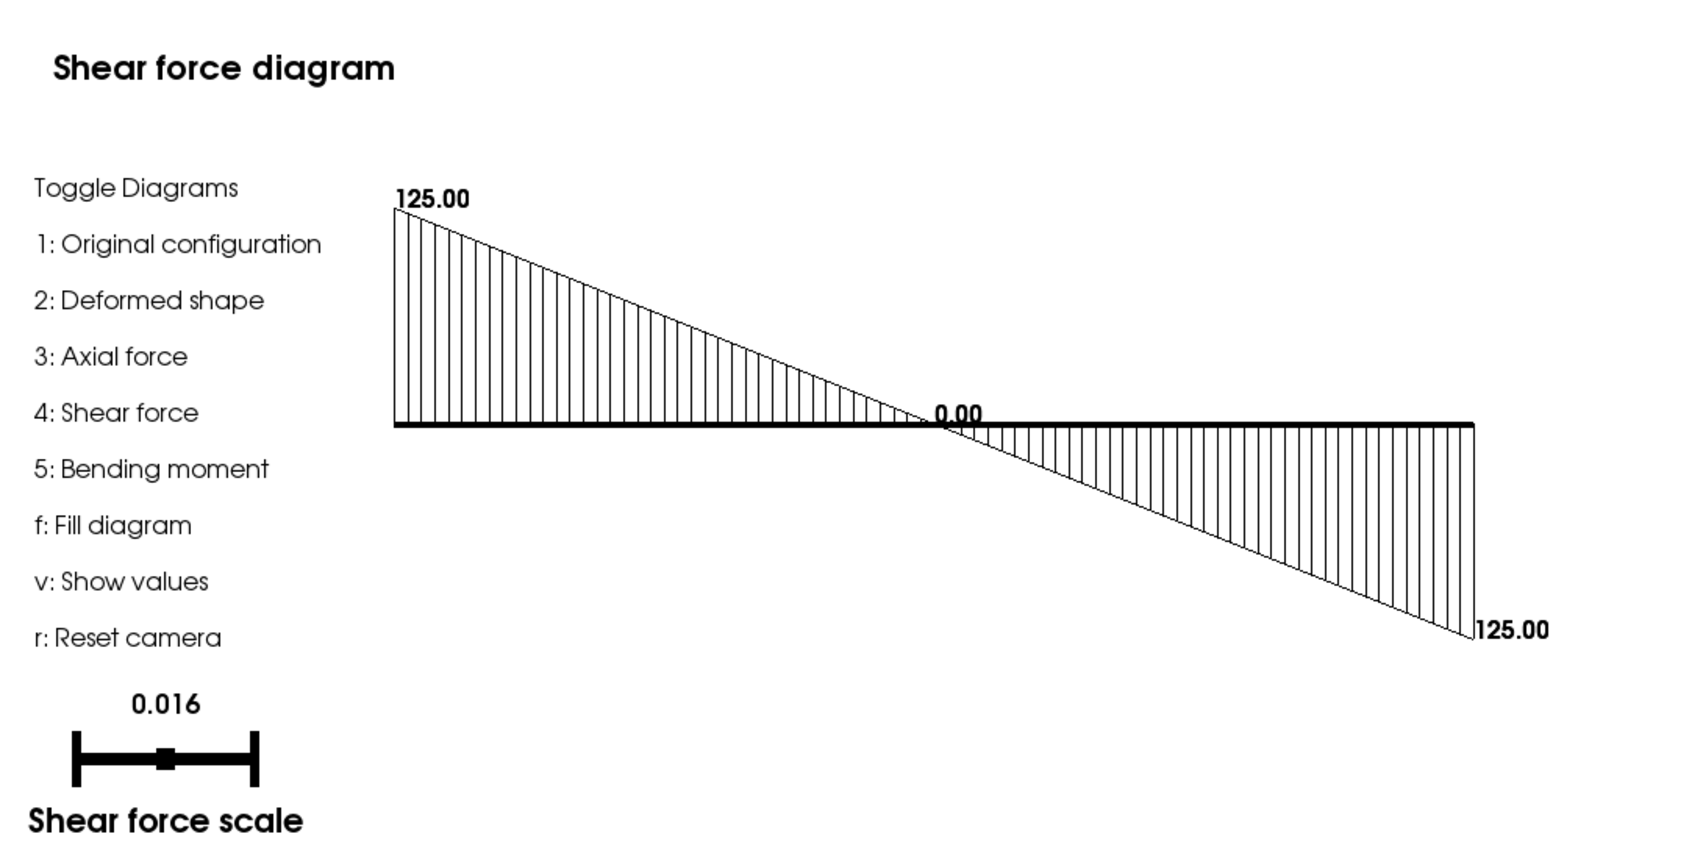
\includegraphics[width=\textwidth, keepaspectratio]{%
                     bm_figures/vtk_figures/bm01_shear.pdf}
    \centering
    \caption{Problem 1, Shear Force Diagram}
    \label{fig:bm01_shear}
\end{figure}
% Moment
\begin{figure}[!htb]
    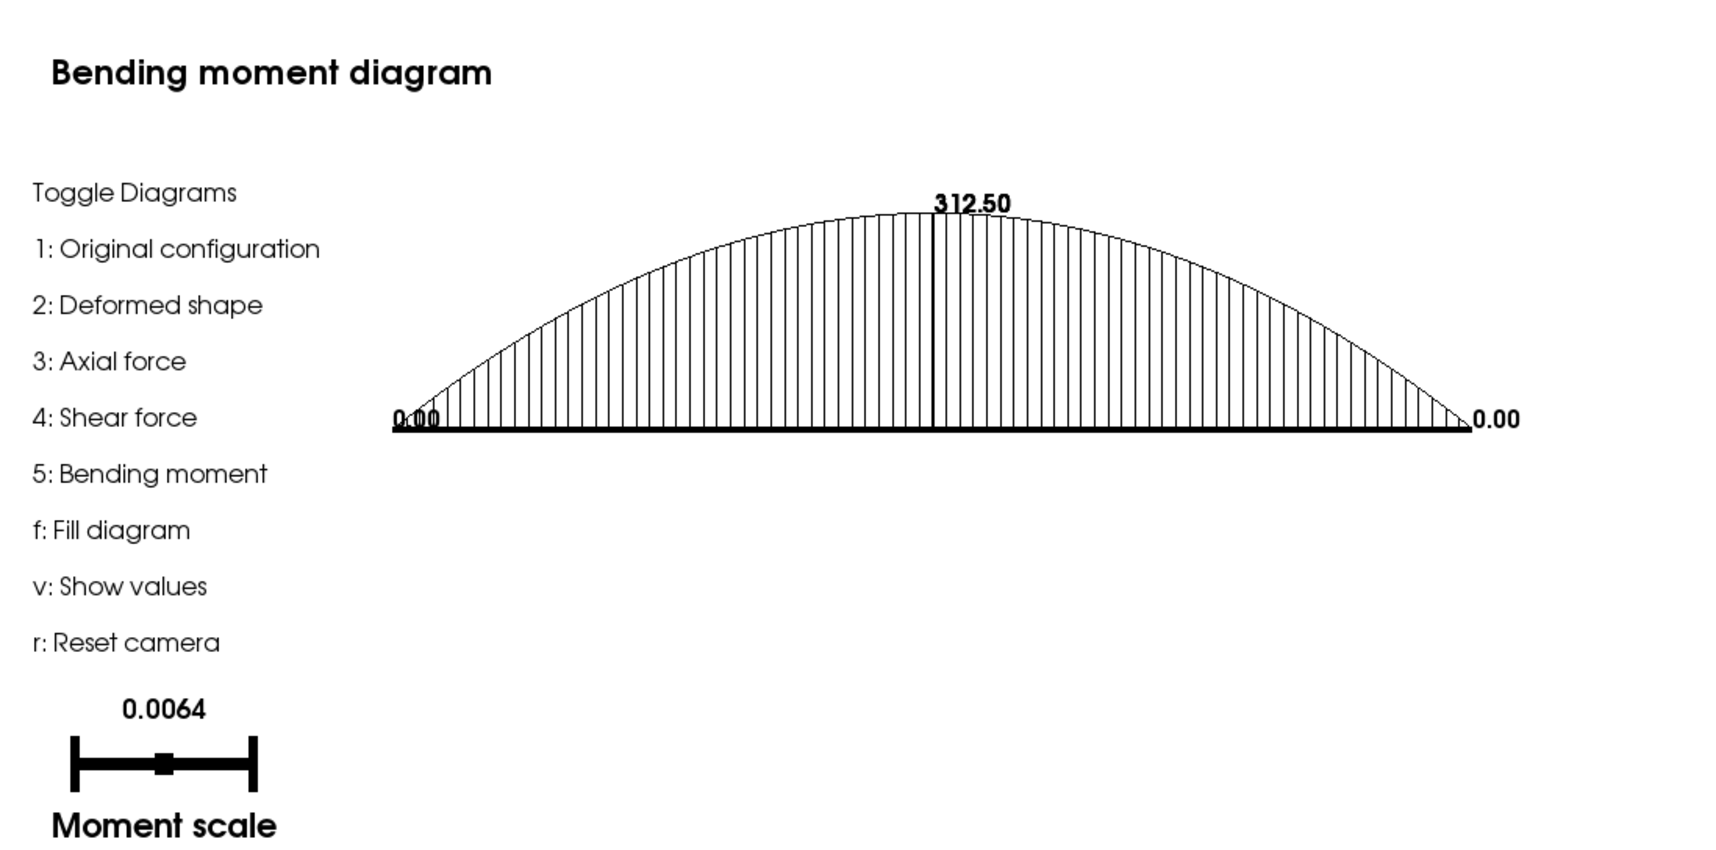
\includegraphics[width=\textwidth, keepaspectratio]{%
                     bm_figures/vtk_figures/bm01_moment.pdf}
    \centering
    \caption{Problem 1, Bending Moment Diagram}
    \label{fig:bm01_moment}
\end{figure}
% Error
\begin{table}[h!]
\centering
\begin{tabular}{ c| c c c c }
    & Exact Expression & Exact Value & Computed Value & \% RE \\ \hline \\
    V   & $\dfrac{\omega l}{2}$ &  125.00 & 125.00 & 0.0\% \\ \\
    $M_{max}$ & $\dfrac{\omega l^2}{8}$ &  312.50 & 312.50 & 0.0\% \\ \\
    $\delta_{max}$ & $\dfrac{5 \omega l^4}{384EI}$ & 0.6357828776E-02 & 0.6357828776E-02 & 0.0\% \\
\end{tabular}
\end{table}

%
% PROBLEM 5
%

\clearpage
\subsubsection{Problem 5: Simple Beam - Load Increasing Uniformly To One End}
\begin{figure}[h]
    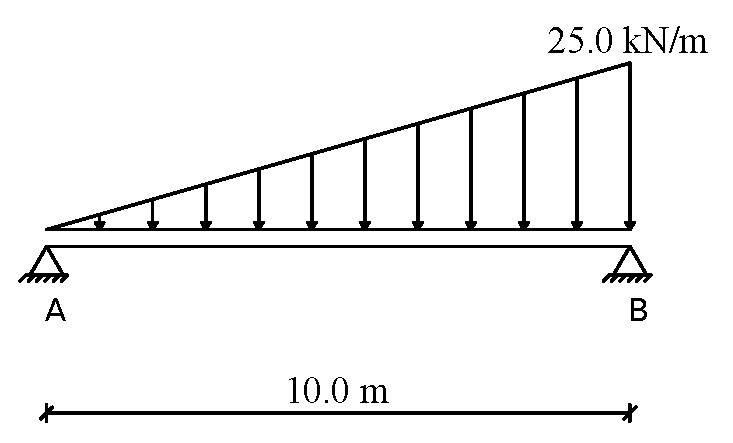
\includegraphics[width=\textwidth, keepaspectratio]{%
                            bm_figures/turtle_figures/bm05_turtle.pdf}
    \centering
    \caption{Problem 5: Loading, geometry and supports}
    \label{fig:bm05_turtle}
\end{figure}
\lstinputlisting{input_files/bm05_input.dat}
\lstinputlisting{output_files/bm05_output.dat}
% Deformed
\begin{figure}[!htb]
    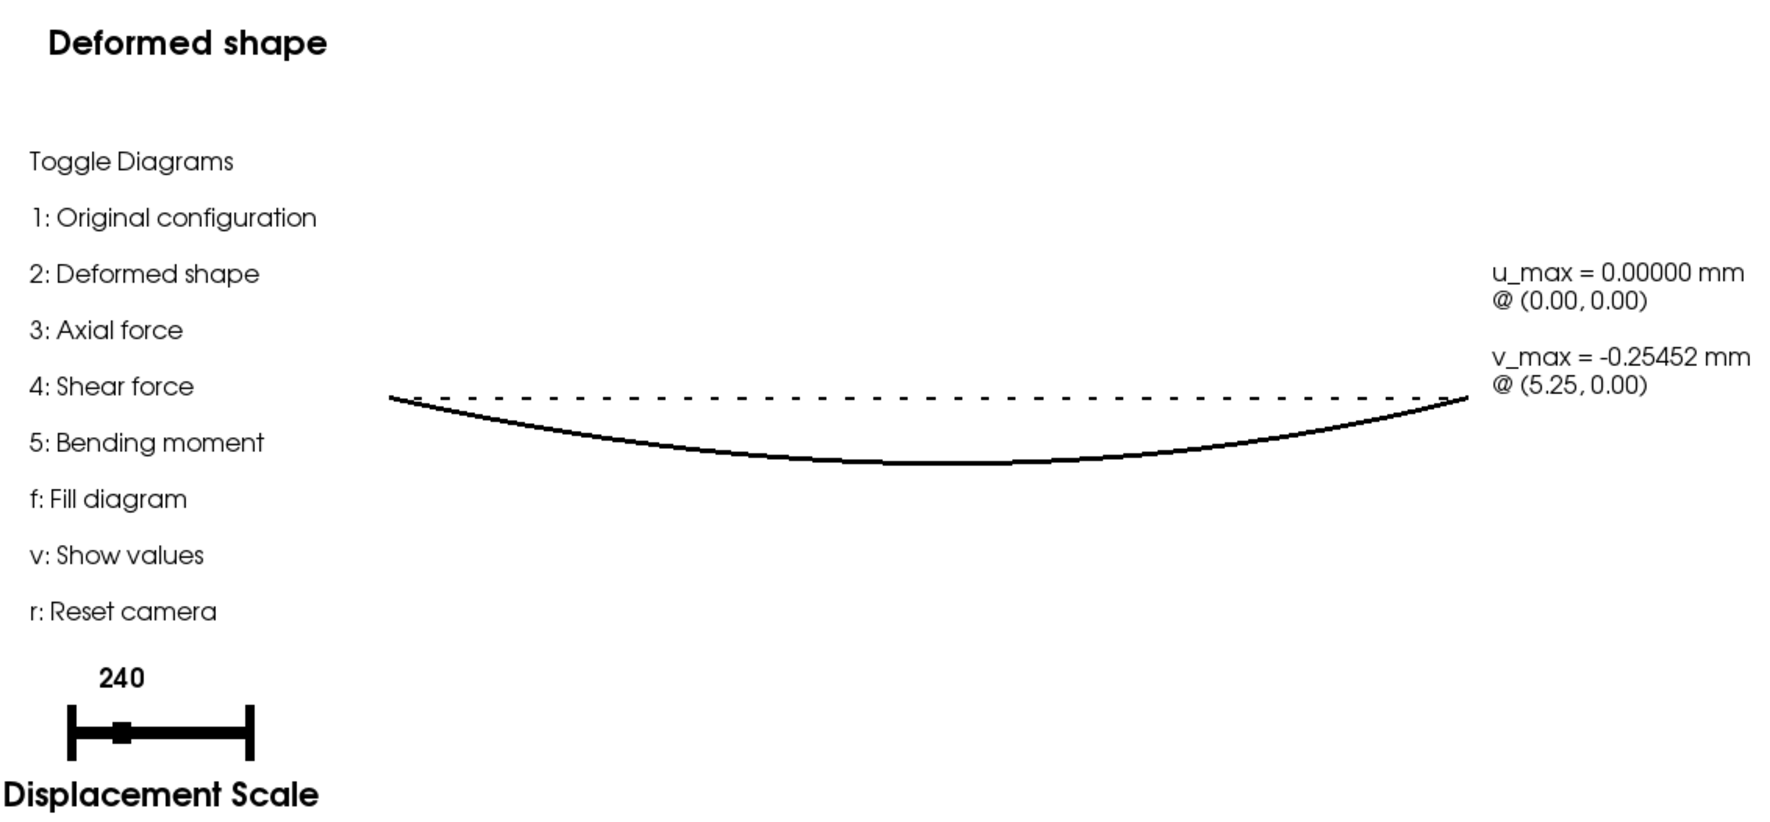
\includegraphics[width=\textwidth, keepaspectratio]{%
                     bm_figures/vtk_figures/bm05_deformed.pdf}
    \centering
    \caption{Problem 5, Deformed Shape}
    \label{fig:bm05_deformed}
\end{figure}
% Shear
\begin{figure}[!htb]
    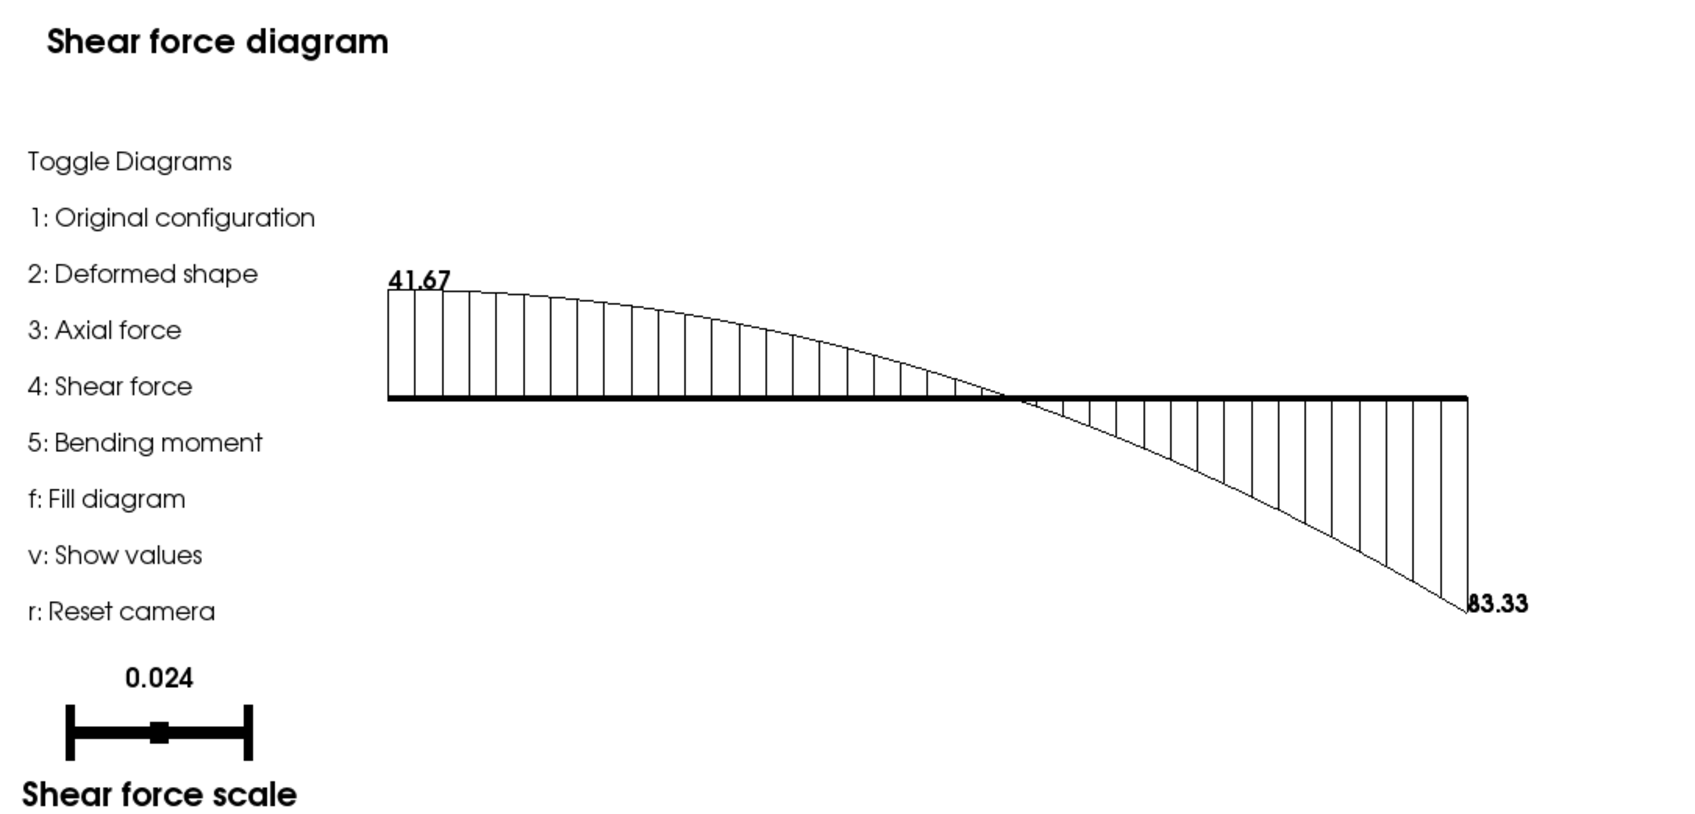
\includegraphics[width=\textwidth, keepaspectratio]{%
                     bm_figures/vtk_figures/bm05_shear.pdf}
    \centering
    \caption{Problem 5, Shear Force Diagram}
    \label{fig:bm05_shear}
\end{figure}
% Moment
\begin{figure}[!htb]
    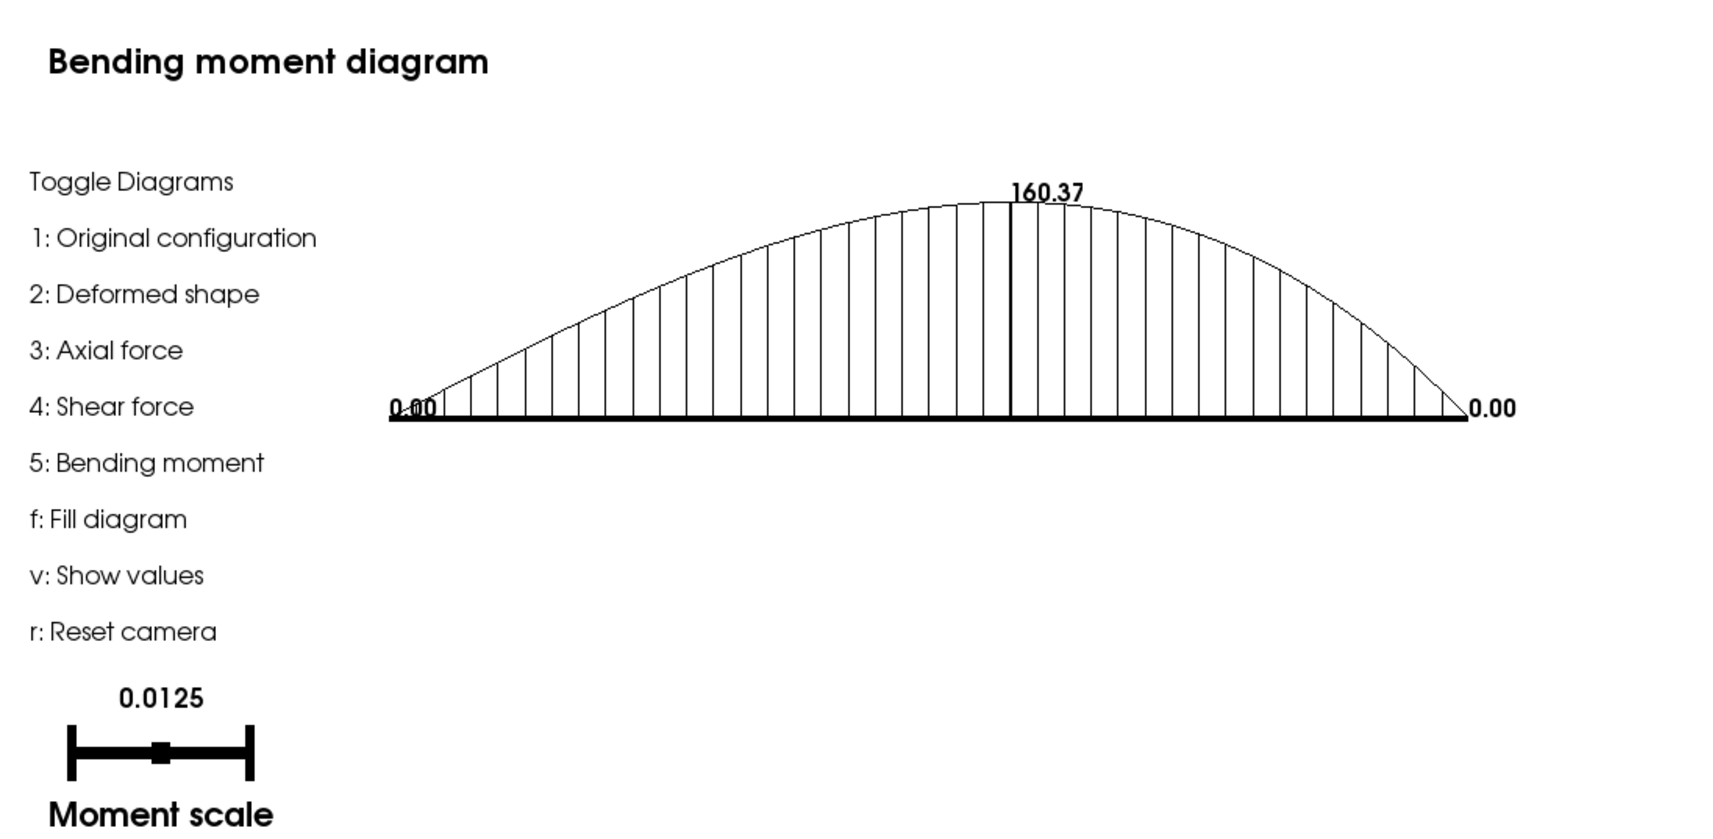
\includegraphics[width=\textwidth, keepaspectratio]{%
                     bm_figures/vtk_figures/bm05_moment.pdf}
    \centering
    \caption{Problem 5, Bending Moment Diagram}
    \label{fig:bm05_moment}
\end{figure}
% Error
\begin{table}[h!]
\centering
\begin{tabular}{ c| c c c c }
    & Exact Expression & Exact Value & Computed Value & \% RE \\ \hline \\
    $V_A$   & $\dfrac{\omega l}{6}$ &  41.67 & 41.67 & 0.0\% \\ \\
    $V_B$  & $\dfrac{ \omega l}{3}$ &  83.33 & 41.67 & 0.0\% \\ \\
    $M_{max}$ & $\dfrac{\omega l^2}{9\sqrt{3}}$ &  160.37 & 160.37 & 0.0\% \\ \\
\end{tabular}
\end{table}

%
% PROBLEM 6
%

\clearpage
\subsubsection{Problem 6: Simple Beam - Load Increasing Uniformly To Center}
\begin{figure}[h]
    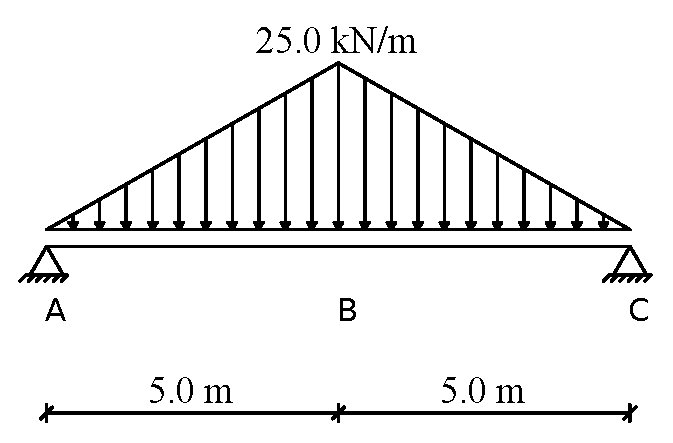
\includegraphics[width=\textwidth, keepaspectratio]{%
                            bm_figures/turtle_figures/bm06_turtle.pdf}
    \centering
    \caption{Problem 6: Loading, geometry and supports}
    \label{fig:bm06_turtle}
\end{figure}
\lstinputlisting{input_files/bm06_input.dat}
\lstinputlisting{output_files/bm06_output.dat}
% Deformed
\begin{figure}[!htb]
    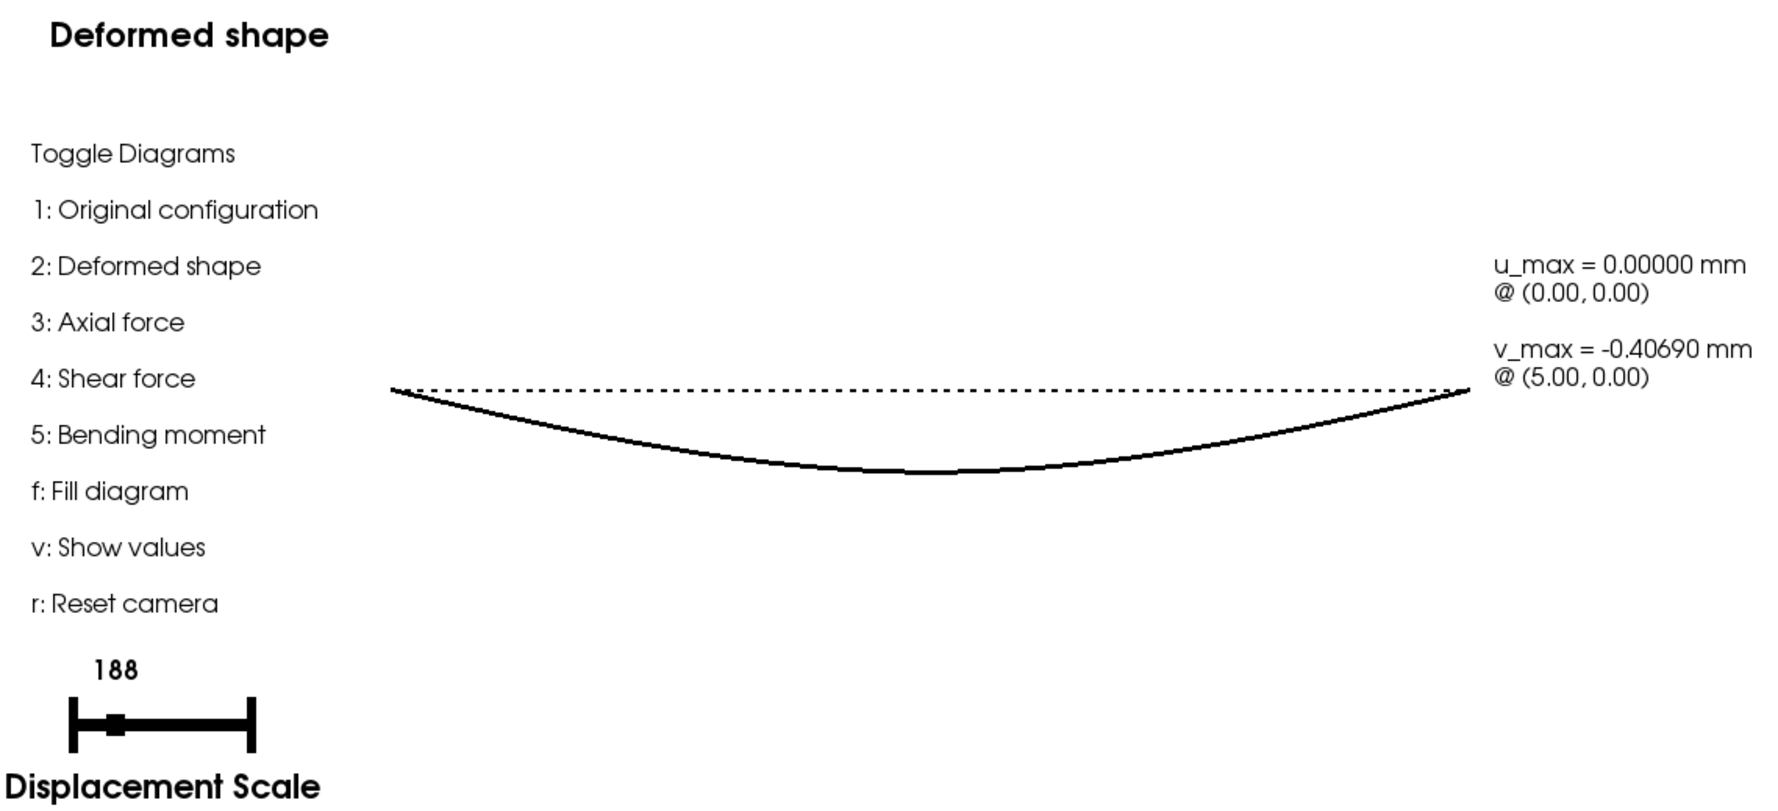
\includegraphics[width=\textwidth, keepaspectratio]{%
                     bm_figures/vtk_figures/bm06_deformed.pdf}
    \centering
    \caption{Problem 6, Deformed Shape}
    \label{fig:bm06_deformed}
\end{figure}
% Shear
\begin{figure}[!htb]
    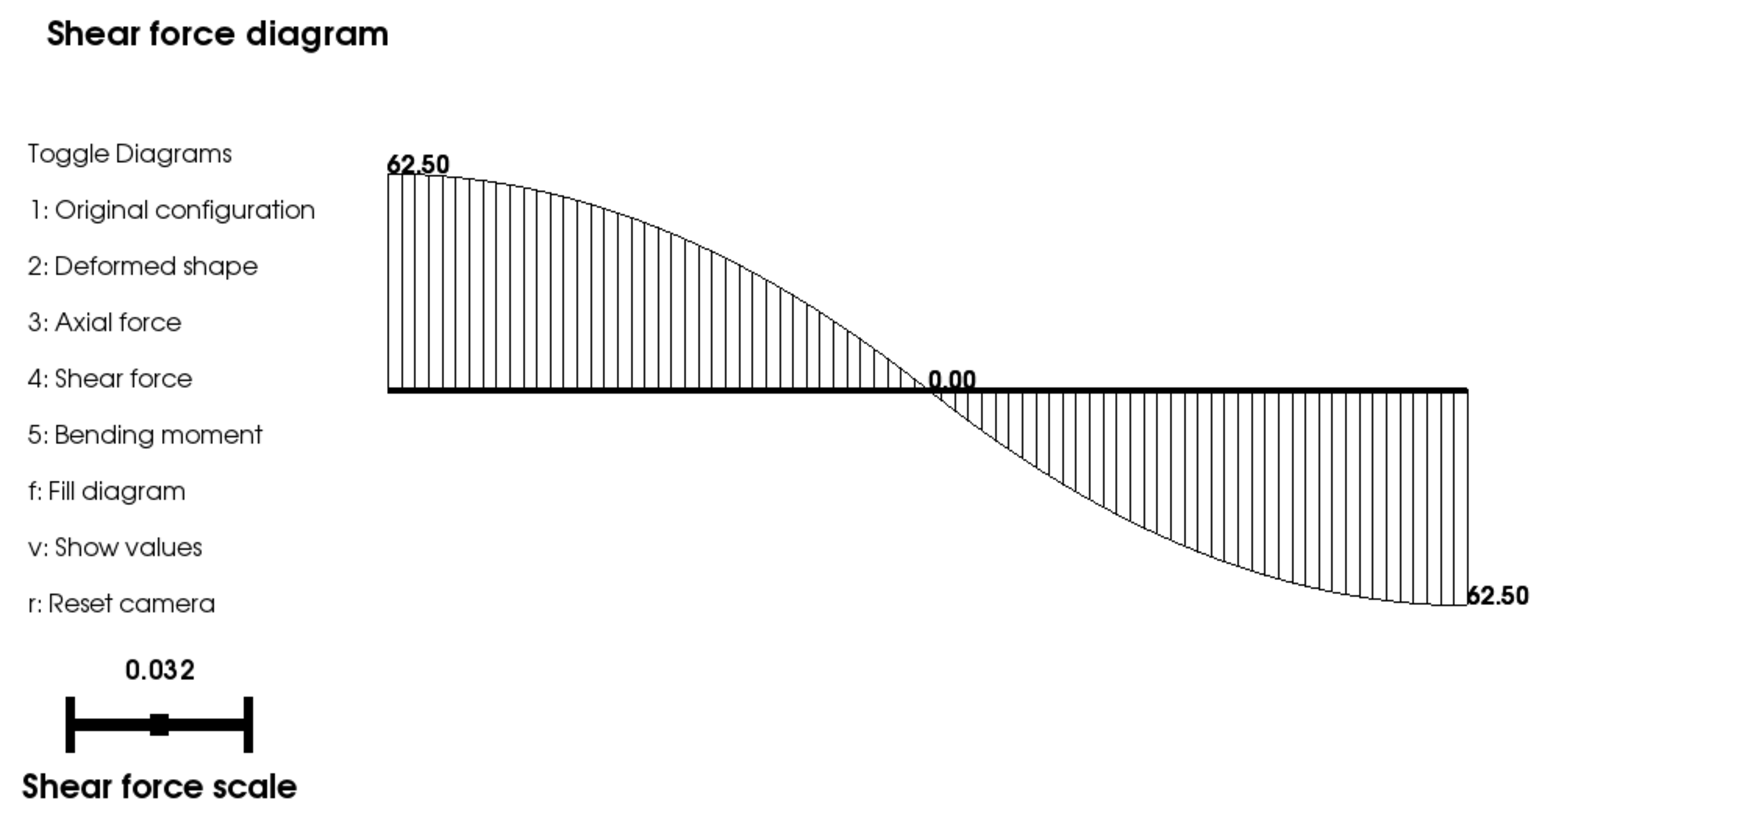
\includegraphics[width=\textwidth, keepaspectratio]{%
                     bm_figures/vtk_figures/bm06_shear.pdf}
    \centering
    \caption{Problem 6, Shear Force Diagram}
    \label{fig:bm06_shear}
\end{figure}
% Moment
\begin{figure}[!htb]
    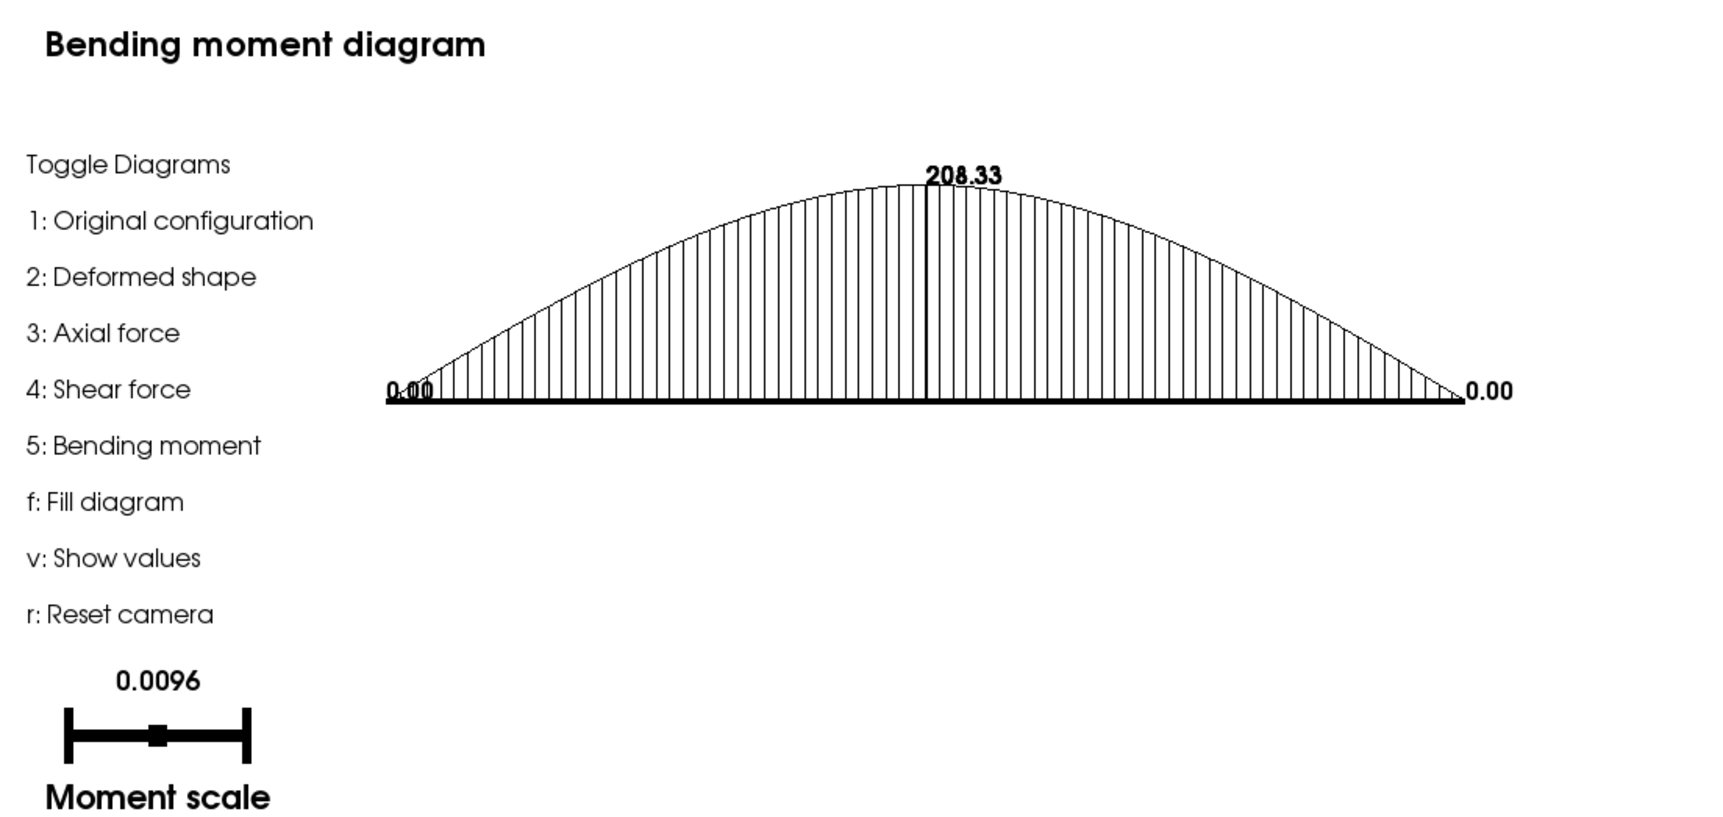
\includegraphics[width=\textwidth, keepaspectratio]{%
                     bm_figures/vtk_figures/bm06_moment.pdf}
    \centering
    \caption{Problem 6, Bending Moment Diagram}
    \label{fig:bm06_moment}
\end{figure}
% Error
\begin{table}[h!]
\centering
\begin{tabular}{ c| c c c c }
    & Exact Expression & Exact Value & Computed Value & \% RE \\ \hline \\
    V   & $\dfrac{\omega l}{4}$ &  62.50 & 62.50 & 0.0\% \\ \\
    $M_{max}$ & $\dfrac{\omega l^2}{12}$ &  208.33 & 208.33 & 0.0\% \\ \\
    $\delta_{max}$ & $\dfrac{\omega l^4}{120EI}$ & 0.4069010417E-02 & 0.4069010417E-02 & 0.0\% \\
\end{tabular}
\end{table}

%
% PROBLEM 9
%

\clearpage
\subsubsection{Problem 9: Simple Beam - Two Equal Concentrated Loads Symmetrically Placed}
\begin{figure}[h]
    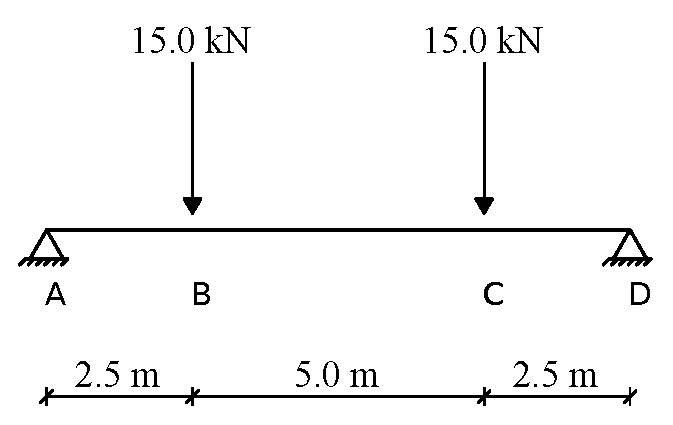
\includegraphics[width=\textwidth, keepaspectratio]{%
                            bm_figures/turtle_figures/bm09_turtle.pdf}
    \centering
    \caption{Problem 9: Loading, geometry and supports}
    \label{fig:bm09_turtle}
\end{figure}
\lstinputlisting{input_files/bm09_input.dat}
\lstinputlisting{output_files/bm09_output.dat}
% Deformed
\begin{figure}[!htb]
    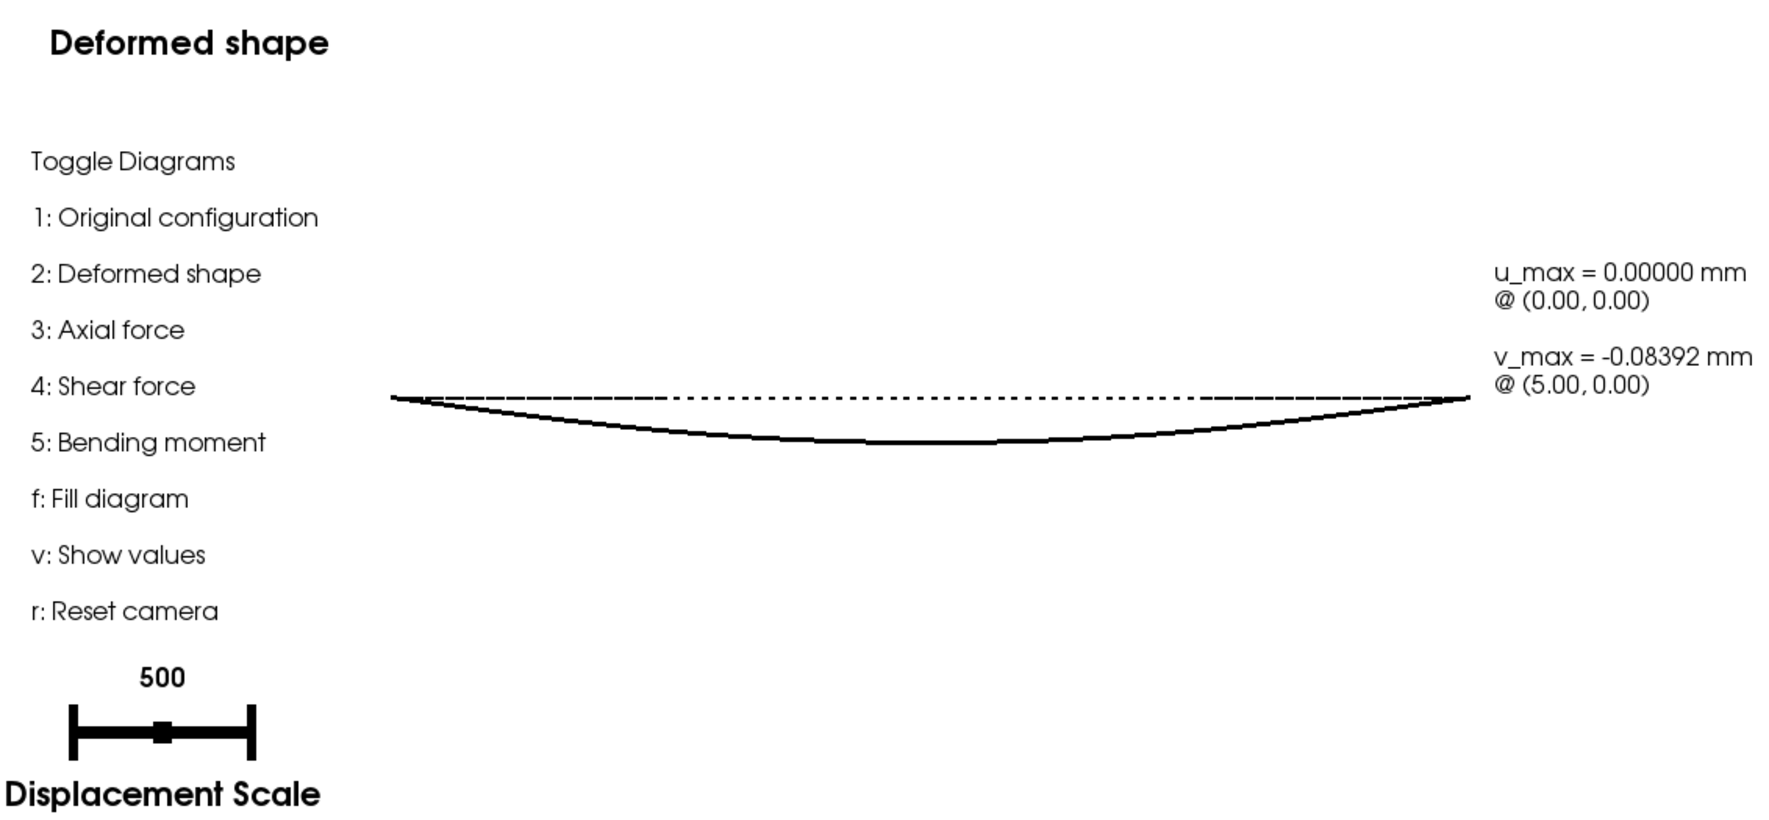
\includegraphics[width=\textwidth, keepaspectratio]{%
                     bm_figures/vtk_figures/bm09_deformed.pdf}
    \centering
    \caption{Problem 9, Deformed Shape}
    \label{fig:bm09_deformed}
\end{figure}
% Shear
\begin{figure}[!htb]
    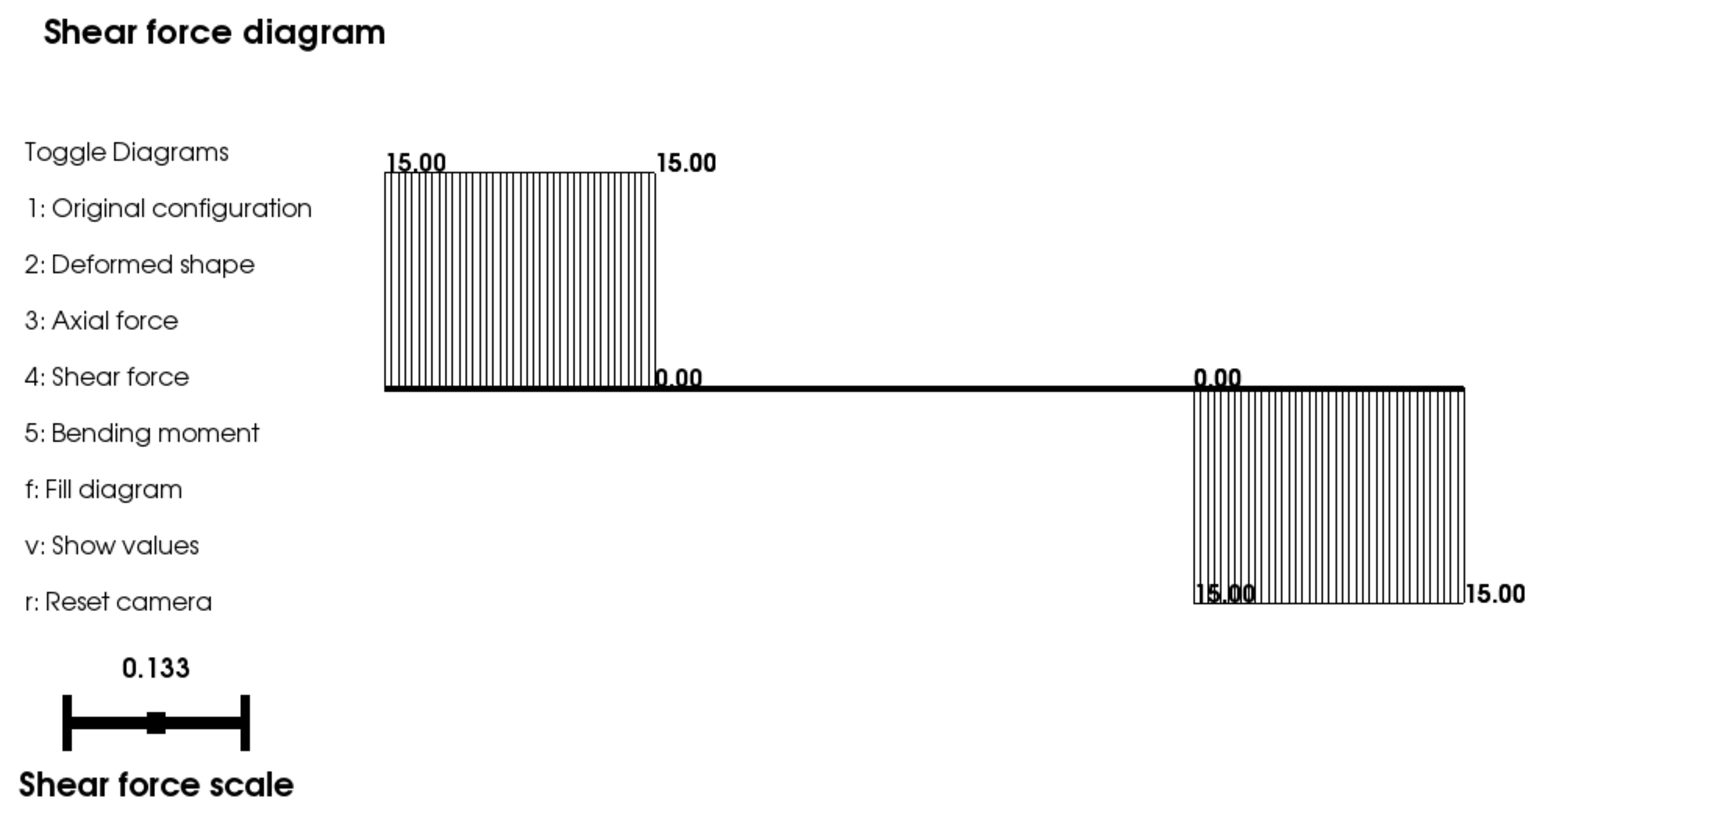
\includegraphics[width=\textwidth, keepaspectratio]{%
                     bm_figures/vtk_figures/bm09_shear.pdf}
    \centering
    \caption{Problem 9, Shear Force Diagram}
    \label{fig:bm09_shear}
\end{figure}
% Moment
\begin{figure}[!htb]
    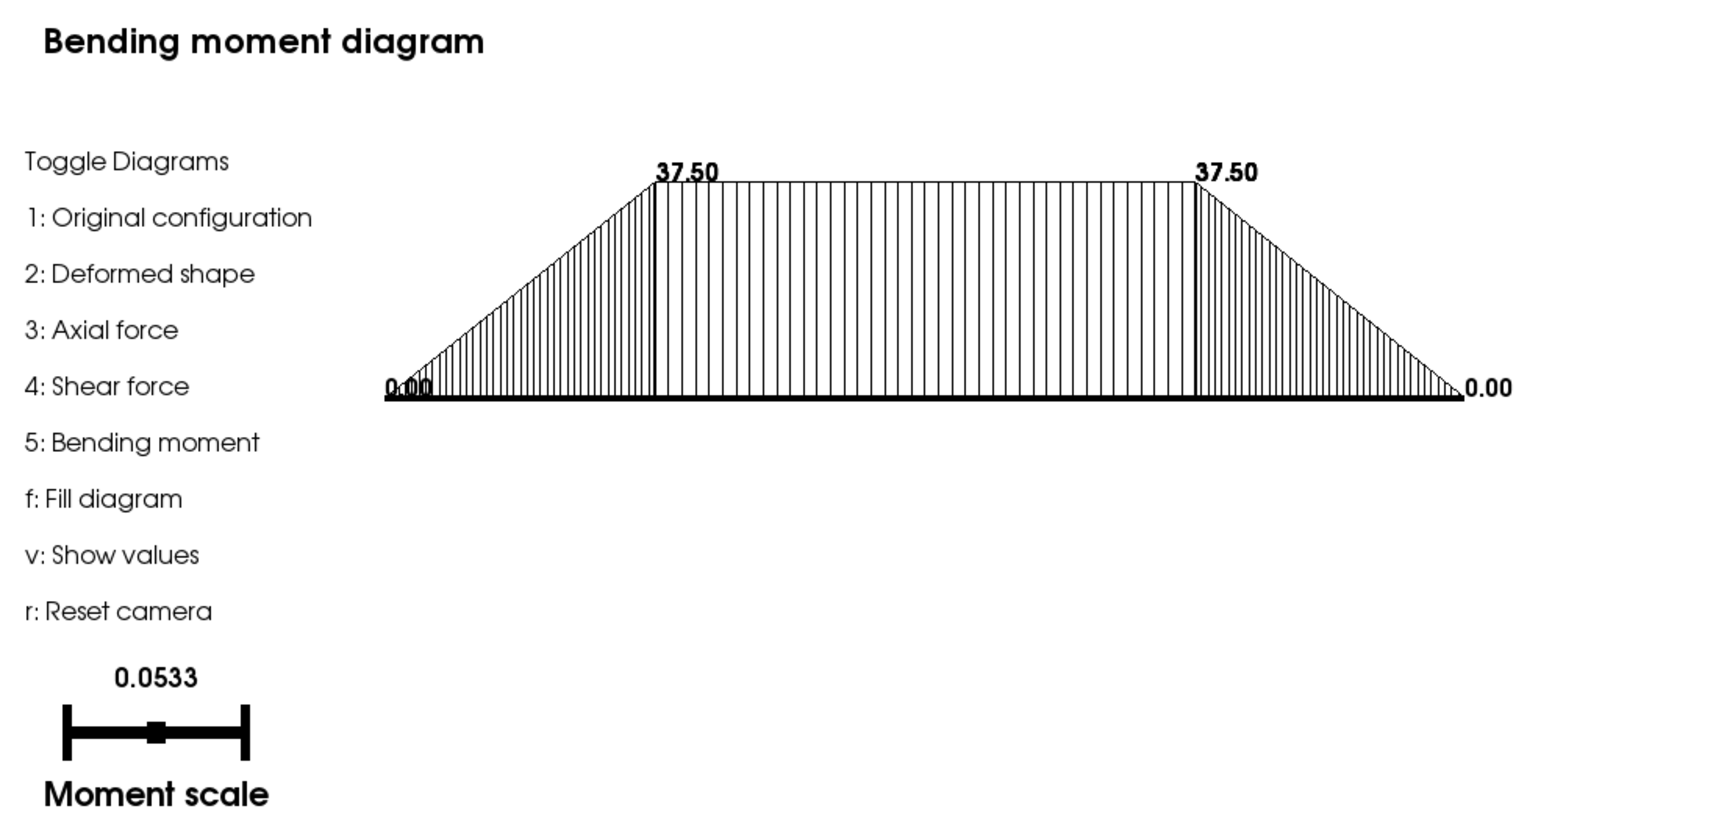
\includegraphics[width=\textwidth, keepaspectratio]{%
                     bm_figures/vtk_figures/bm09_moment.pdf}
    \centering
    \caption{Problem 9, Bending Moment Diagram}
    \label{fig:bm09_moment}
\end{figure}
% Error
\begin{table}[h!]
\centering
\begin{tabular}{ c| c c c c }
    & Exact Expression & Exact Value & Computed Value & \% RE \\ \hline \\
    V   & P & 15.00 & 15.00 & 0.0\% \\ \\
    $M_{max}$ & Pa & 37.50 & 37.50 & 0.0\% \\ \\
    $\delta_{max}$ & $\dfrac{Pa}{24EI}(3l^2 - 4a^2)$ & 0.8392333984E-03 & 0.8392333984E-03 & 0.0\% \\
\end{tabular}
\end{table}

%
% PROBLEM 14
%

\clearpage
\subsubsection{Problem 14: Cantilever Beam - Concentrated Load At Any Point}
\begin{figure}[h]
    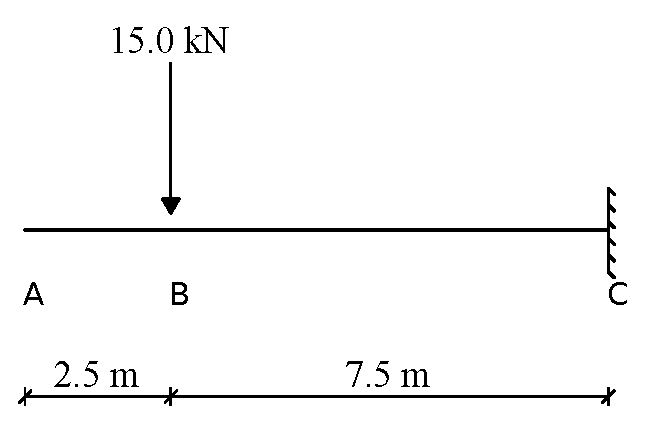
\includegraphics[width=\textwidth, keepaspectratio]{%
                            bm_figures/turtle_figures/bm14_turtle.pdf}
    \centering
    \caption{Problem 14: Loading, geometry and supports}
    \label{fig:bm14_turtle}
\end{figure}
\lstinputlisting{input_files/bm14_input.dat}
\lstinputlisting{output_files/bm14_output.dat}
% Deformed
\begin{figure}[!htb]
    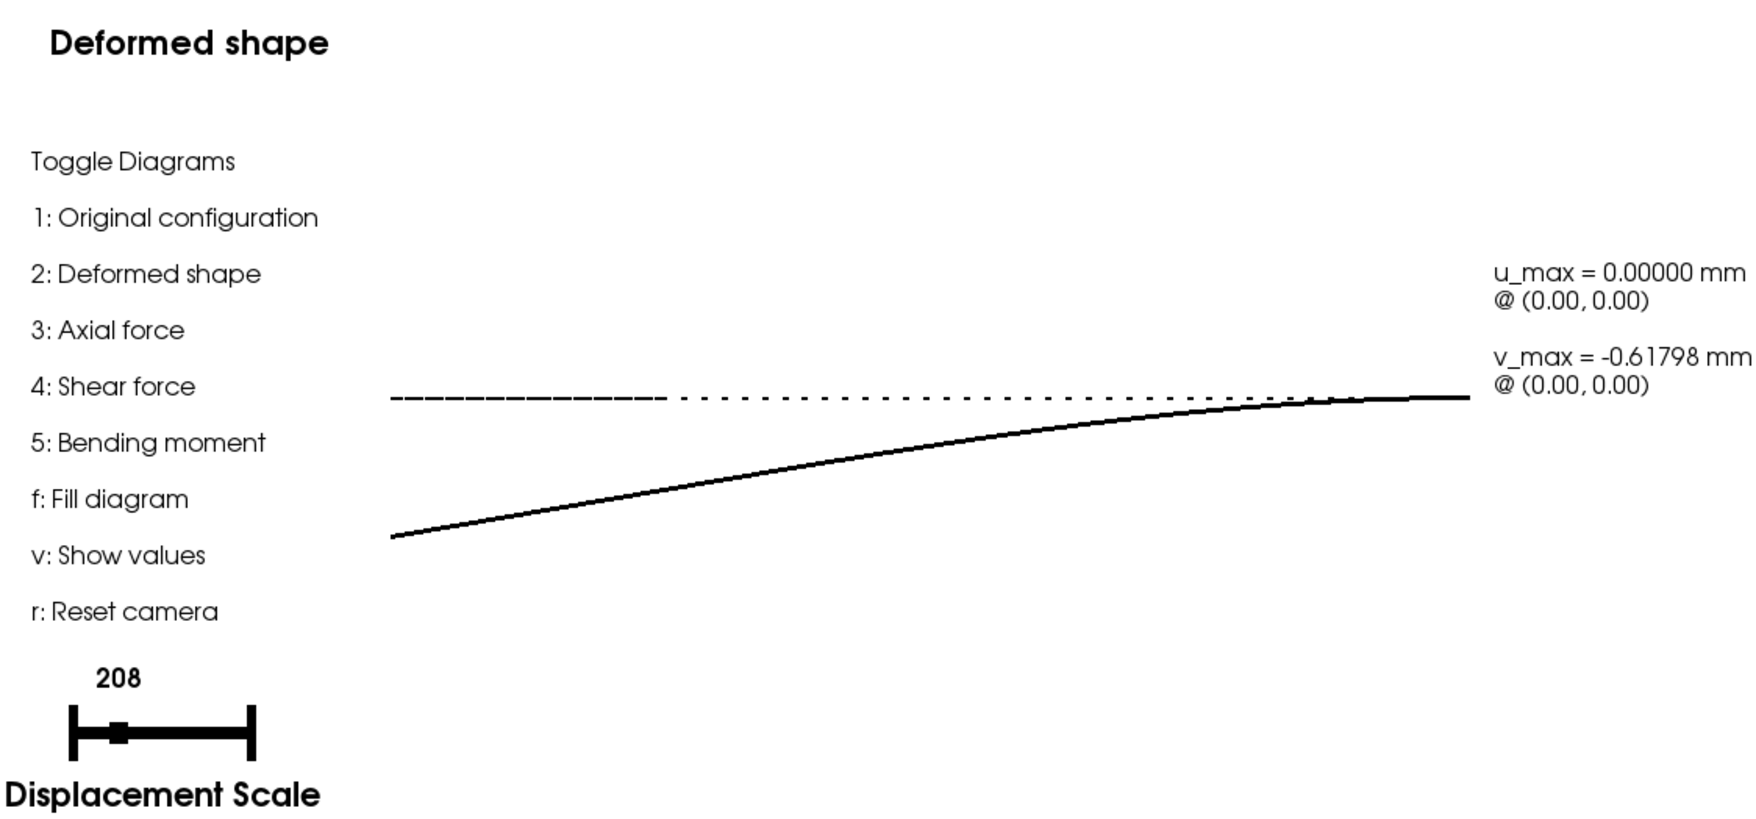
\includegraphics[width=\textwidth, keepaspectratio]{%
                     bm_figures/vtk_figures/bm14_deformed.pdf}
    \centering
    \caption{Problem 14, Deformed Shape}
    \label{fig:bm14_deformed}
\end{figure}
% Shear
\begin{figure}[!htb]
    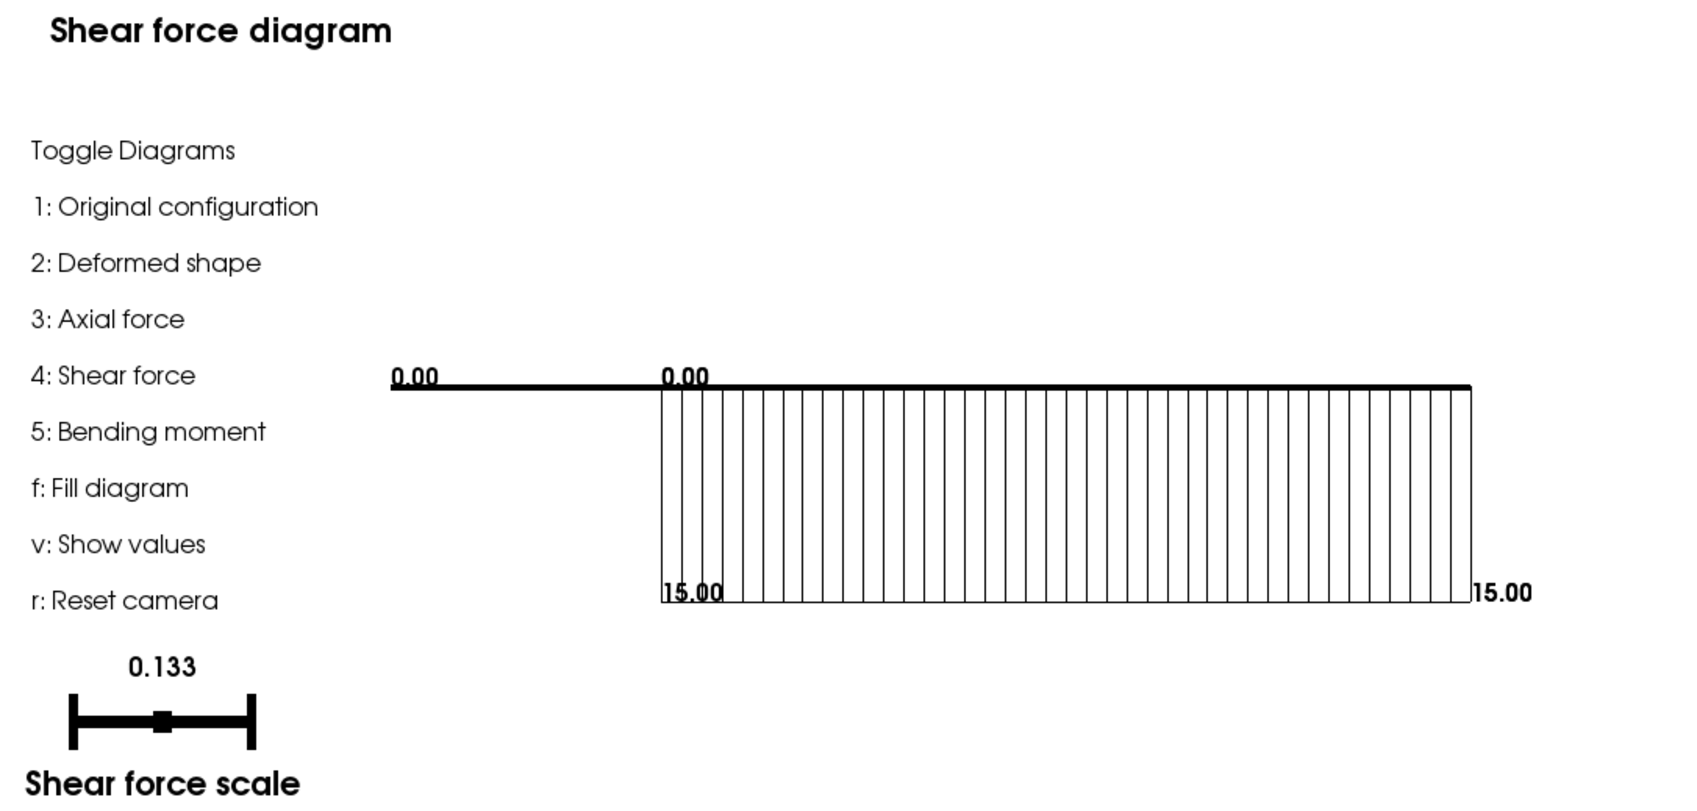
\includegraphics[width=\textwidth, keepaspectratio]{%
                     bm_figures/vtk_figures/bm14_shear.pdf}
    \centering
    \caption{Problem 14, Shear Force Diagram}
    \label{fig:bm14_shear}
\end{figure}
% Moment
\begin{figure}[!htb]
    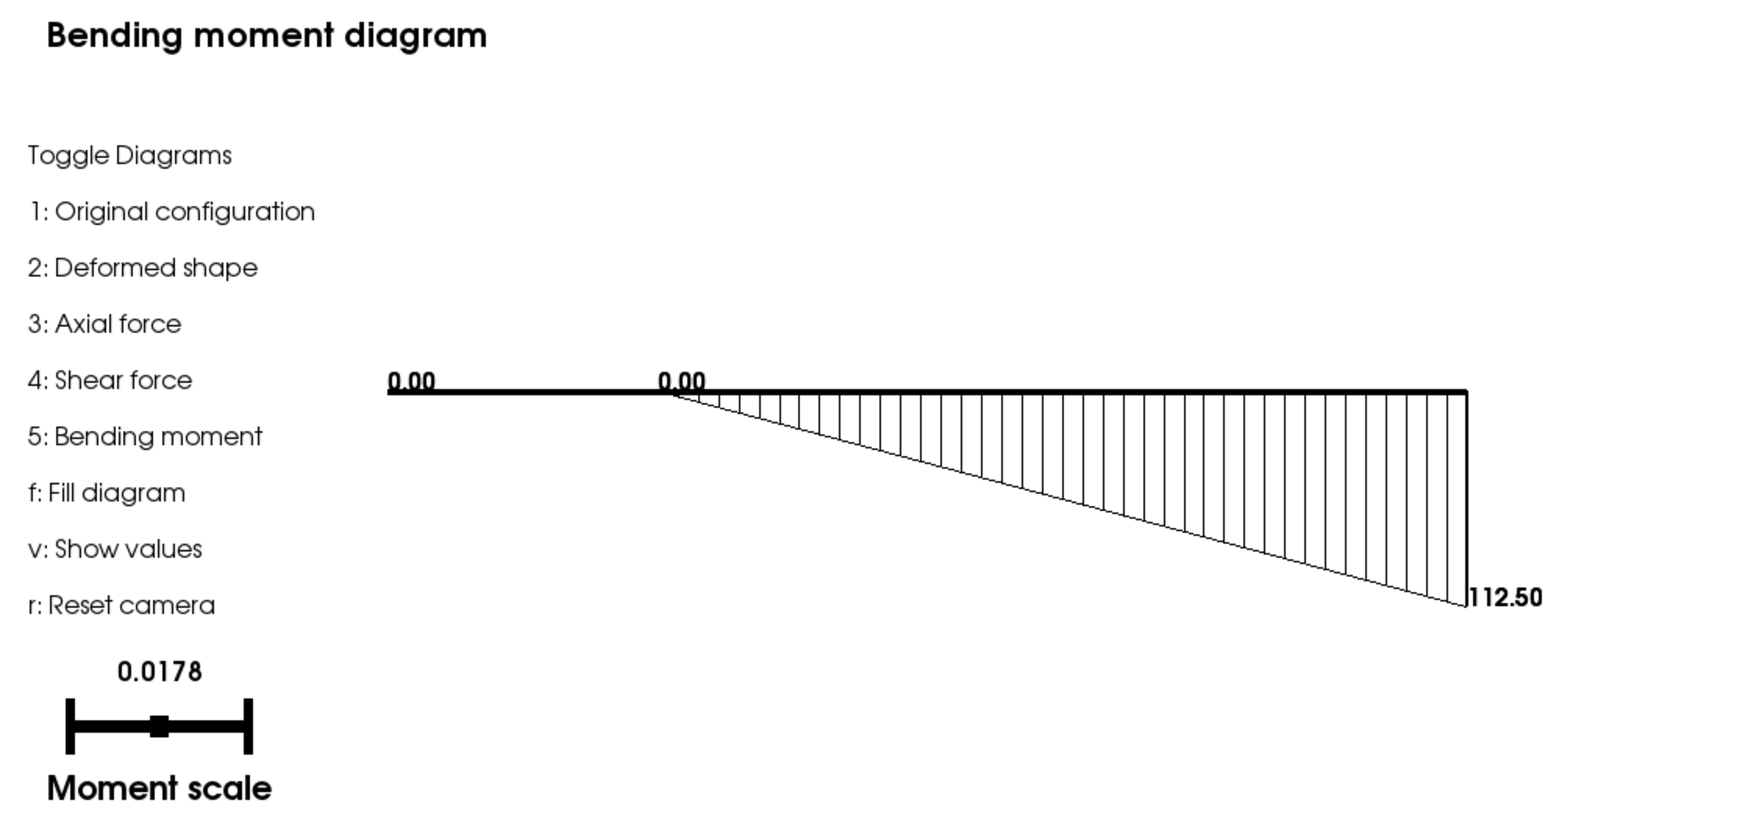
\includegraphics[width=\textwidth, keepaspectratio]{%
                     bm_figures/vtk_figures/bm14_moment.pdf}
    \centering
    \caption{Problem 14, Bending Moment Diagram}
    \label{fig:bm14_moment}
\end{figure}
% Error
\begin{table}[h!]
\centering
\begin{tabular}{ c| c c c c }
    & Exact Expression & Exact Value & Computed Value & \% RE \\ \hline \\
    V   & P & 15.00 & 15.00 & 0.0\% \\ \\
    $M_{max}$ & Pb & 112.50 & 112.50 & 0.0\% \\ \\
    $\delta_{max}$ & $\dfrac{Pb**2}{6EI}(3l-b)$ & 0.6179809570E-02 & 0.6179809570E-02 & 0.0\% \\
    $\delta_{B}$ & $\dfrac{Pb**3}{3EI}$ & 0.4119873047E-02 & 0.4119873047E-02 & 0.0\% \\
\end{tabular}
\end{table}

